\section{Основная часть}
\subsection{Датасет CIFAR-10}
Набор данных, на котором проводились исследования, состоит из 60\,000 цветных изображений, размера 
32$\times$32 пикселя. Каждое изображение принадлежит одному из 10 классов, что соответствует 600 изображениям на класс. Под 
обучение отводится 50\,000 изображений. Остальные 10\,000 используются для тестирования. Объекты в классах сильно варьируются, 
например, класс <<птица>> содержит различные виды птиц, как большие так и маленькие. Кроме того, объекты классов представлены в 
различных позах и под различными углами. Особенно это проявляется среди собак и котов, которые изображены не только в различных 
позах, но иногда и частично, например, изображена только голова животного.

Датасет CIFAR-10 \cite{learningmultiple} был выбран для проведения исследований благодаря своему относительно небольшому размеру, 
который позволяет обучать глубокие нейронные сети используя GPU с памятью меньше 8\,Gb, например, в данном работе использовалась 
NVIDIA Grid K520 с 4\,Gb видеопамяти.

На момент написания работы лучший результат (state-of-the-art) на CIFAR-10 составляет 96.53\% \cite{2014arXiv1412}. Точность  
распознавания человека приблизительно равна 
94\%.\footnote{\url{http://karpathy.github.io/2011/04/27/manually-classifying-cifar10/}}

\begin{figure}[h]
\centering
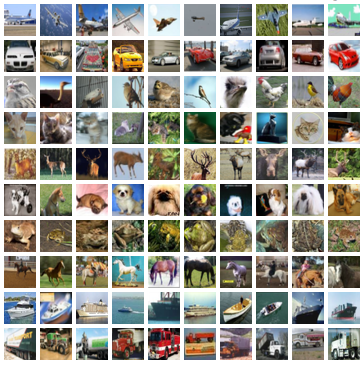
\includegraphics[width=0.5\textwidth]{cifar10}
\caption{10 случайных изображений из каждого класса CIFAR-10}
\end{figure}

\subsection{Фреймворк Caffe}
Обучение нейронных сетей проводилось с использованием фреймворка для глубокого обучения Caffe \cite{jia2014caffe}.
Изначально, фреймворк разрабатывался командой BVLC (Berkeley Vision and Learning Center), но постепенно перерос в большой 
open-source проект.\footnote{\url{https://github.com/BVLC/caffe}} На данный момент вклад в развитие Caffe внесли почти 200 
разработчиков и более 10\,000 человек оценили проект на Github.

Данный фреймворк был выбран для решения задачи по нескольким причинам:
\begin{enumerate}
    \item Простота определения моделей и методов оптимизации. Топологии нейронных сетей и алгоритмы оптимизации определяются в 
    специальных конфигурационных файлах типа Google Protocol 
    Buffers.\footnote{\url{https://developers.google.com/protocol-buffers/}} Caffe поддерживает топологии сетей в форме любых 
    ациклических графов.
    \item Модульность. Caffe позволяет легко изменять архитектуру сети под новые форматы входных данных. Кроме того, в наличии 
    имеется много слоёв и функций потерь.
    \item Скорость вычислений и эффективное использование ресурсов. Caffe заранее выделяет ровно столько памяти сколько нужно для 
    нейронной сети. Помимо этого, для операций c примитивами линейной алгебры Caffe использует BLAS (Basic Linear Algebra 
    Subroutines), а для операций свёртки и матричного умножения библиотеку cuDNN \cite{DBLP:journals/corr/ChetlurWVCTCS14}. 
    \item Интерфейсы для Python и Matlab.
\end{enumerate}

Caffe написан на языках C++, Cuda, Python. Для хранения больших объёмов данных используются базы данных 
LMDB\footnote{\url{http://symas.com/mdb/}} и LevelDB\footnote{\url{https://github.com/google/leveldb}}. Обучение нейронных сетей 
может производиться как на CPU, так и на нескольких GPU одновременно. Фреймворк доступен для установки на Linux, Windows и OS X.
\subsection{Предварительная обработка данных}
\subsection{Обучение нейронных сетей}
\subsection{Анализ результатов одиночных моделей}
\subsection{Объединение нейронных сетей в ансамбль}